% Seven legal circular words of length 4, in rotation piles of sizes 1, 4 and 2.
% Positions run clockwise from the top: 1, 2, 3, 4. Rust disc = 1, open disc = 0.
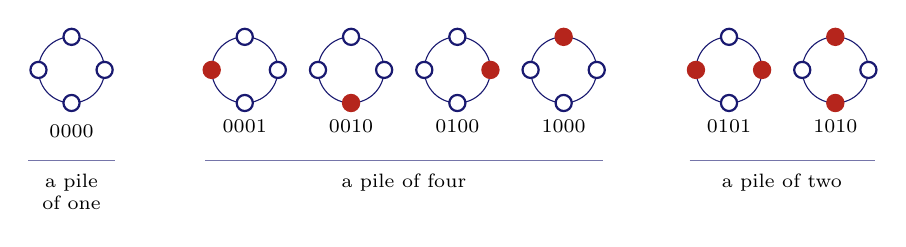
\begin{tikzpicture}[x=1cm,y=1cm,
  off/.style={circle,draw=MidnightBlue,thick,fill=white,inner sep=0pt,minimum size=2.05mm},
  on/.style={circle,draw=BrickRed,thick,fill=BrickRed,inner sep=0pt,minimum size=2.05mm}]
  % all zeros
  \draw[MidnightBlue,thin] (0,0) circle (0.42);
  \node[off] at (0,0.42) {};
  \node[off] at (0.42,0) {};
  \node[off] at (0,-0.42) {};
  \node[off] at (-0.42,0) {};
  \node[font=\scriptsize,anchor=north] at (0,-0.58) {$0000$};

  % one 1, rotated
  \draw[MidnightBlue,thin] (2.2,0) circle (0.42);
  \node[off] at (2.2,0.42) {};
  \node[off] at (2.62,0) {};
  \node[off] at (2.2,-0.42) {};
  \node[on] at (1.78,0) {};
  \node[font=\scriptsize] at (2.2,-0.72) {$0001$};

  \draw[MidnightBlue,thin] (3.55,0) circle (0.42);
  \node[off] at (3.55,0.42) {};
  \node[off] at (3.97,0) {};
  \node[on] at (3.55,-0.42) {};
  \node[off] at (3.13,0) {};
  \node[font=\scriptsize] at (3.55,-0.72) {$0010$};

  \draw[MidnightBlue,thin] (4.9,0) circle (0.42);
  \node[off] at (4.9,0.42) {};
  \node[on] at (5.32,0) {};
  \node[off] at (4.9,-0.42) {};
  \node[off] at (4.48,0) {};
  \node[font=\scriptsize] at (4.9,-0.72) {$0100$};

  \draw[MidnightBlue,thin] (6.25,0) circle (0.42);
  \node[on] at (6.25,0.42) {};
  \node[off] at (6.67,0) {};
  \node[off] at (6.25,-0.42) {};
  \node[off] at (5.83,0) {};
  \node[font=\scriptsize] at (6.25,-0.72) {$1000$};

  % period 2
  \draw[MidnightBlue,thin] (8.35,0) circle (0.42);
  \node[off] at (8.35,0.42) {};
  \node[on] at (8.77,0) {};
  \node[off] at (8.35,-0.42) {};
  \node[on] at (7.93,0) {};
  \node[font=\scriptsize] at (8.35,-0.72) {$0101$};

  \draw[MidnightBlue,thin] (9.7,0) circle (0.42);
  \node[on] at (9.7,0.42) {};
  \node[off] at (10.12,0) {};
  \node[on] at (9.7,-0.42) {};
  \node[off] at (9.28,0) {};
  \node[font=\scriptsize] at (9.7,-0.72) {$1010$};

  \draw[MidnightBlue!60] (-0.55,-1.15) -- (0.55,-1.15);
  \node[font=\scriptsize,anchor=north,align=center] at (0,-1.2) {a pile\\of one};
  \draw[MidnightBlue!60] (1.7,-1.15) -- (6.75,-1.15);
  \node[font=\scriptsize,anchor=north] at (4.22,-1.2) {a pile of four};
  \draw[MidnightBlue!60] (7.85,-1.15) -- (10.2,-1.15);
  \node[font=\scriptsize,anchor=north] at (9.02,-1.2) {a pile of two};
\end{tikzpicture}
